%%%%%%%%%%%%%%%%%%%%%%%%%%%%%%%%%%%%%%%%%
% FRI Data Science_report LaTeX Template
% Version 1.0 (28/1/2020)
%
% Jure Demšar (jure.demsar@fri.uni-lj.si)
%
% Based on MicromouseSymp article template by:
% Mathias Legrand (legrand.mathias@gmail.com)
% With extensive modifications by:
% Antonio Valente (antonio.luis.valente@gmail.com)
%
% License:
% CC BY-NC-SA 3.0 (http://creativecommons.org/licenses/by-nc-sa/3.0/)
%
%%%%%%%%%%%%%%%%%%%%%%%%%%%%%%%%%%%%%%%%%


%----------------------------------------------------------------------------------------
%	PACKAGES AND OTHER DOCUMENT CONFIGURATIONS
%----------------------------------------------------------------------------------------
\documentclass[fleqn,moreauthors,10pt]{ds_report}
\usepackage[english]{babel}
\usepackage{float}
\graphicspath{{fig/}}




%----------------------------------------------------------------------------------------
%	ARTICLE INFORMATION
%----------------------------------------------------------------------------------------

% Header
\JournalInfo{UL FRI Data Science - Introduction to Data Science, 2021-2022}

% Interim or final report
\Archive{Final report}
%\Archive{Project X Report}

% Article title
\PaperTitle{Product recommendation system}

% Authors and their info
%\Authors{David Ocepek, Klementina Pirc, Matej Miočić\textsuperscript{1}}
%\affiliation{\textsuperscript{1}\textit{mm9520@student.uni-lj.si, 63180206}}

% Multiple authors
\Authors{David Ocepek\textsuperscript{1}, Klementina Pirc\textsuperscript{2} and Matej Miočić\textsuperscript{3}}
\affiliation{\textsuperscript{1}\textit{do8572@student.uni-lj.si, 63160248}}
\affiliation{\textsuperscript{2}\textit{kp3437@student.uni-lj.si, 63210492}}
\affiliation{\textsuperscript{3}\textit{mm9520@student.uni-lj.si, 63180206}}

% Keywords
\Keywords{recommendation system, products, RankFM, DeepFM}
\newcommand{\keywordname}{Keywords}


%----------------------------------------------------------------------------------------
%	ABSTRACT
%----------------------------------------------------------------------------------------

\Abstract{
The goal of our project was to build a product recommendation system that would help the sales personnel at Siemens recommend more relevant products to their customers. We have evaluated 2 models (RankFM and DeepFM) that were trained on information about customer previous purchases and compared the results to the baseline model. We approached the evaluation from different standpoints and the trained model managed to outperform the baseline model in all of them. When evaluating the models based on hit-rate, the top hit@5 rate for RankFM was 0.68 compared to top hit@5 rate for baseline model which was 0.44. This means that the RankFM model correctly predicted at least 1 out of 5 predicted products for almost 25\% more users than the baseline model. 
}

% For our project we evaluated 1st and 2nd order FM's, DeepFM, LSTM-DeepFM and compared them with the popular RankFM library.
% The RankFM library outperformed all other models indicating that there are some optimizations in the library which are crucial to model performance.
% The top hit@5 rate for RankFM was 0.66 indicating on average 3 out of 5 customer will be interested in purchasing at least one of the five recommended products.
% Currently DeepFM achieved a hit@5 rate of 0.52 and was slightly better than 1st and 2nd order FM's, this lead us to conclude that indicating that if similar sampling methods used to the RankFM achieve a hit rate of above 0.66.
% We also used a probability threshold to remove items with low probabilities achieving an improvement in the F1 score for all models.
% }

%----------------------------------------------------------------------------------------

\begin{document}

% Makes all text pages the same height
\flushbottom

% Print the title and abstract box
\maketitle

% Removes page numbering from the first page
\thispagestyle{empty}

%----------------------------------------------------------------------------------------
%	ARTICLE CONTENTS
%----------------------------------------------------------------------------------------

\section*{Introduction}
Sales performance is one of the most important aspects of businesses therefore a lot of effort goes into its advancement. Suggesting new popular products or products adjusted to customers' needs contributes to mentioned goals and this is where recommendation systems are utilised. Our goal was to create a recommendation system for Siemens that provided us with information about their customer purchases. For the task we resorted to  Factorisation Machines (RankFM) and Deep Factorisation Machines (DeepFM) that are specialised for recommendations and are therefore designed to learn from sparse data which is one of the characteristics of recommendation problems. Below we describe utilised methods and present our results.

%Recommendation systems as they are known however pose a set of unique and complex challenges to solve. Firstly, they are almost universally sparse, since we will have a large number of products and customers, but each customer is expected to buy a non-zero but nonetheless very small portion of items.
% The aforementioned is a big problem for most algorithms since they cannot learn from sparse data and it requires us to use algorithms specialised for recommendation such as Matrix Factorisation (MF), Factorisation Machines (FM), Deep Factorisation Machines (DeepFM) or some even more sophisticated methods such as Graph Neural Network (GNN).

%Another problem that becomes quickly apparent is the lack of negative samples, meaning examples of when customers didn't buy anything.
%These are important but often times hard to acquire simply because it requires companies to not only log successful purchases but also customer enthusiasm for a product which they latter did not buy, this is often hard or even infeasible and when possible care is required to interpret the negative samples.
%It may be tempting to omit negative samples altogether, however it has been shown that most models perform better if they have access to data on customer behaviour not just when the prior made a purchase, but also when he decided not purchase anything.


%Our report is structured as follows: firstly we give a brief rundown of our key data analysis takeaways, then we explain our models and how we pre-processed our data, afterwards we present our results, which we then discuss, we conclude our report by giving key takeaways Siemens can use such as proposed libraries, models to use and improvements to said models.

%----------sent the methodology----, then we pre----------ly a------, final------------------

\section*{Data analysis}

Our data set consists of 1249 consecutive days for which we have information about product sales for each customer. Given attributes are: \textit{day, customer, prod, domestic, state, ind\_code, ind\_seg\_code, new\_orders}. \textit{5HB8\_4N50\_1I6D} is an example of a product label, where \textit{5HB8} is the family, \textit{4N50} the product and \textit{1I6D} product's variation. Same product and variation labels appear in different families, therefore we were attentive to also include family label when carrying out analysis and predictions. Data set contains 2762 customers, 126 families, 2013 products and 12304 variations. Additionally we have some information about each customer: their industry and industry segmentation code, whether they are a domestic customer (from Austria) or not and which state the customer is from. These features are uniquely determined by the customer id, something which is important as it enables us to impute said features in our negative samples. Starting date of the data set is assumed to be sometime in the late spring or early summer. We deducted this from Figure~\ref{top} which shows a clear seasonality in our data characterised by sharp periodic drops in sales.

\begin{figure}[hbt]\centering
	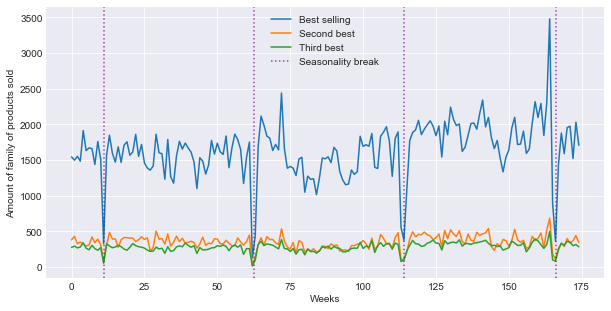
\includegraphics[width=\linewidth]{top_products.png}
	\caption{Amount of sales for \textbf{top 3 families of products} through time. Seasonality of our dataset can be seen in the form of periodic drops and lifts in sales. The figure also shows a clear dominance of the most popular family of products.}
	\label{top}
\end{figure}

In \noindent Figure \ref{top} we show a clear dominance in sales of the most popular family of products. We observe that the most frequently bought family of products has approximately three times as much sales as the second most frequently bought family of products, with second and third being similar, leading us to conclude that most families have expected sales similar to the bottom two families.

\begin{figure}[H]\centering
	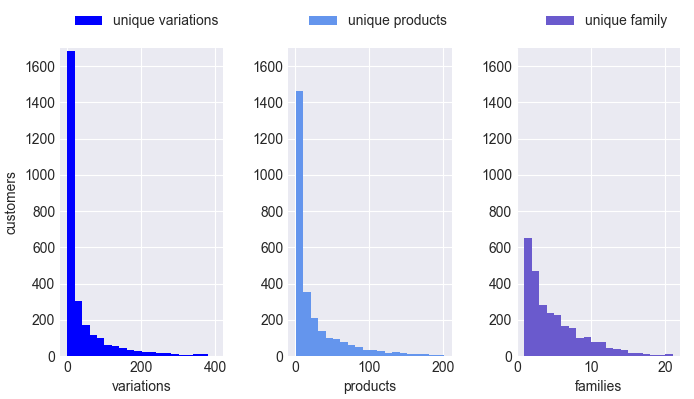
\includegraphics[width=\linewidth]{unique.png}
	\caption{Distribution of unique families, products and variations per customer. Most customers only buy a few select product variations.}
	\label{unique}
\end{figure}

\noindent From Figure~\ref{unique} we conclude that our prediction rate (even for a constant classifier) should be quite high due to the small number of purchases made by each customer as such most of our classification problem stems not from accurately assessing which items a customer will buy, but instead when a customer will buy a certain product.

\section*{Methods}

\subsection*{Walk-forward cross-validation}

\noindent We are working with temporal data and the model must not learn from the future data, therefore we decided to use walk-forward cross-validation (WF-CV), which is a technique that splits the data into folds and at the same time preservers the temporal ordering of the data. We decided to use 500 days as train data and 125 days as test data, this allows us to go through all the data in 6 folds (Figure \ref{cv}). 

\begin{figure}[H]\centering
	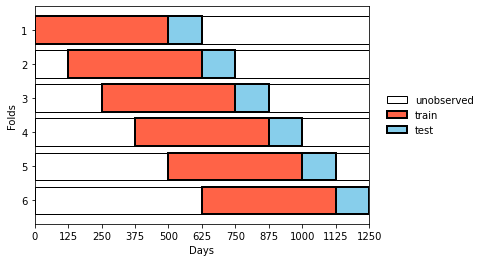
\includegraphics[width=\linewidth]{cv.png}
	\caption{\textbf{Walk-forward cross-validation.} All folds have equal amounts of data, the train and the test set include 500 and 125 days respectively.}
	\label{cv}
\end{figure}

\subsection*{Hyperparameter tunning}
To determine the optimal values of hyperparameters for our models we applied nested cross validation, with grid search inside each fold. In each fold of nested CV we performed holdout estimation for each parameter in grid, choosing the parameters which minimised our mean squared error (MSE).

\subsection*{Feature Embedding}
Most recommender systems use some form of feature embedding to reduce high-dimensional customer-product feature spaces and extract valuable information from our data. This approach is used by FM, DeepFM or LSTM.
All three models learn feature embeddings during training.

\subsection*{Negative sampling}
Examples of when customers didn't buy anything (negative samples) can be hard to acquire because it requires companies to also log customer's enthusiasm for a product which they did not buy. We could omit negative samples altogether, however it has been shown that most models perform better if they have access to data on customer behaviour not just when they make a purchase, but also when they decide not to purchase anything. We used a one-to-one negative sample ratio with uniform distribution across all customer-product pairs. 

\subsection*{The baseline model}
The baseline model is important for understanding the true performance of our models. Baseline values for predictions are calculated by picking the most frequent family for each customer, based on their purchases in the train set, then predicting top $k$ variations or products from this family and finally checking if the customer bought any of them in the future (test set). Family prediction is done independent of customers by always using top $k$ families from the train set.

\subsection*{Factorization Machines}
Factorization Machines (FM) are a family of supervised learning algorithms that map arbitrary real-valued features into a low-dimensional latent factor space and can be applied naturally to a wide variety of prediction tasks including regression, classification, and ranking. FMs can estimate model parameters accurately under very sparse data and train with linear complexity, allowing them to scale to very large data sets — these characteristics make FM an ideal fit for real-world recommendation problems. Additionally we can set the complexity of FM, in practice the most commonly used are 1st and 2nd order FM which are also the two options that we evaluated in our work~\cite{fm}.

\subsection*{RankFM}
RankFM\footnote{\url{https://github.com/etlundquist/rankfm}} is a cython implementation of the FM model adapted for collaborative filtering recommendation/ranking problems with implicit feedback user/item interaction data. For user implicit data we used user's state, where as for item implicit data we used from which family each product is. However we are not able to utilise explicit data such as the exact day and the amount of items purchased.

\subsection*{DeepFM}
Deep Factorisation Machines~\cite{DeepFM} (DeepFM) are an improvement over FM, combining FM with deep neural networks (DNN), which enables the model not to only predict sparse features but also model higher degree non-linear interactions which FM struggle with as they can usually model only 1st and 2nd order polynomial feature interaction.
Another benefit of using DeepFM is the huge expressiveness offered by neural networks.
In our paper we used a vanilla deep neural network.

DeepFM and its components (mainly 1st and 2nd order FM) were implemented in Keras.
Our personal implementations of these models enabled us to compare our model performances with the performance of popular library models.

\subsection*{Hit rate}
For estimating the performance of our models we used the hit-rate measure. If a customer buys at least one of the $k$ recommended products in the test set it counts as a hit. Finally, we calculated the portion of customers for which we got a hit. For recommending 5 products per user we denote hit rate as top hit@5 rate.

\subsection*{F1-score}
Instead of predicting a fixed number of products for each customer, another approach is to focus only on products whose probability is higher than a given threshold. This functionality was specifically requested by Siemens so the sales person can set a certain threshold and recommend only products that a customer will be very likely be interested in. In this case we estimated the performance of our models with the F1-score as it represents the harmonic mean between precision and recall. To calculate predictions we took 10 recommended products and filtered out items below the threshold, then calculated true positives (\textbf{TP}) - correctly recommended items, false positives (\textbf{FP}) - incorrectly recommended items and false negatives (\textbf{FN}) - items users bought but were not recommended. With obtained results we calculated precision (\textbf{Pr}), recall (\textbf{Re}), combining them into the \textbf{F1-score} (\ref{eq2}), as follows

%\begin{equation}
%	 Precision = \frac{TP}{(TP + FP)}, \ Recall = \frac{TP}{(TP + FN)},
%	\label{eq1}
%\end{equation}

\begin{equation}
	 F1 = \frac{2 \cdot precision \cdot recall}{precision + recall} = \frac{TP}{TP + \frac{1}{2}(FP + FN)}.
	\label{eq2}
\end{equation}

\noindent To further illustrate why we think F1-score is a better metric for this approach we created a simple example in Figure \ref{4}. In this example a user has bought 3 items (A,B,C) in the test set (shown on the left). We recommend 5 items (X,B,C,D,E) and slowly increase the threshold, such that 1 less item is recommended in each row. If the filtered out recommendation was incorrect, precision and with that F1-score increases, meanwhile hit-rate stays the same (first 3 rows). When we reach a threshold, where we filter out correct recommendations, precision and with that F1-score decreases (4th row). Only when we filter out all correct recommendations the F1-score and hit-rate evaluate to 0 (bottom row).

\begin{figure}[H]\centering
	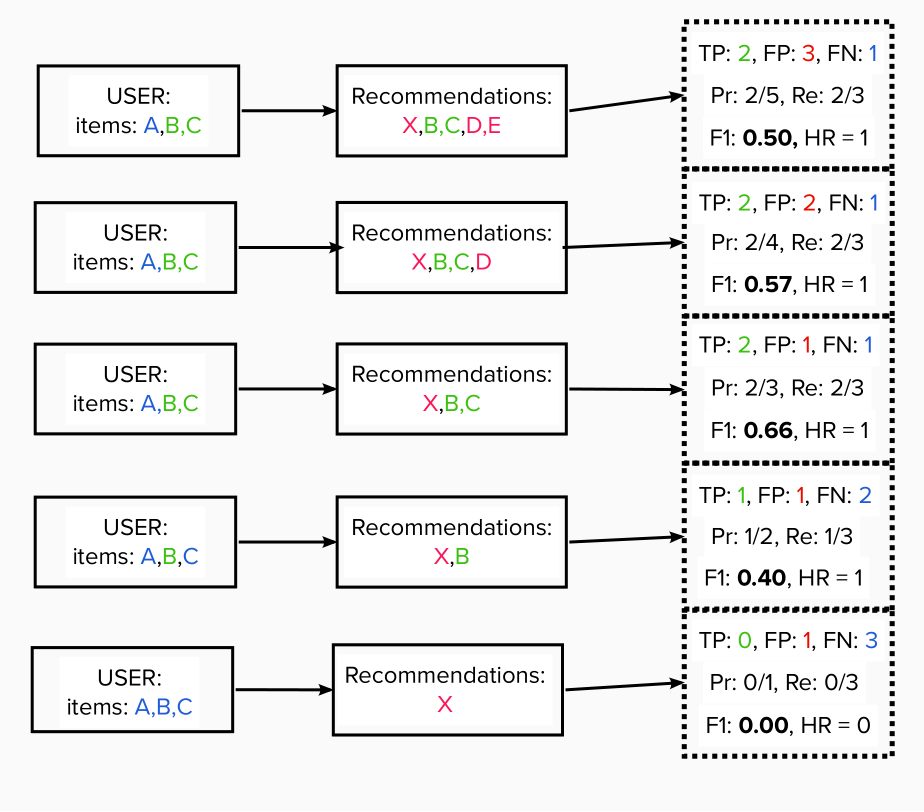
\includegraphics[width=0.9\linewidth]{example.png}
	\caption{\textbf{A visualisation of evaluation metrics} illustrating why we think F1-score is a better metric than hit-rate when recommending based on probabilities, where TPs are labeled in green, FPs in red and FNs in blue. The left column shows the items that each user bought, the middle one recommendations and the right one shows calculated F1-scores and hit rates for different recommendations.} 
	\label{4}
\end{figure}

\section*{Results}

\subsection*{Hyperparameter search}
A subset of the most important tunned hyperparameter is shown in Table~\ref{tab:hyper-corr}.
The subset includes the dimension of our embeddings (k), model learning rates (lr), L1, L2 and dropout regularization (dr).
All models were tunned using a Grid of parameter and if the optimal parameters were on the border of our search space, we increased its size guaranteeing that we found a minimum.
\begin{table}[hbt]
    \centering
    \begin{tabular}{c|c|c|c|c|c|c}
        Parameter & k & lr & dr & L1 & L2 \\
        \hline
        RankFM & 40 & 0.3 & - & - & 0.01 \\
        Order 2 FM & 50 & 1e-5 & - & 0.0 & 1e-4\\
        DeepFM & 50 & 1e-3 & 0.3 & 0.0 & 0.0\\
    \end{tabular}
    \caption{Optimal parameters for validation.}
    \label{tab:hyper-corr}
\end{table}

\begin{figure*}[h!]\centering
	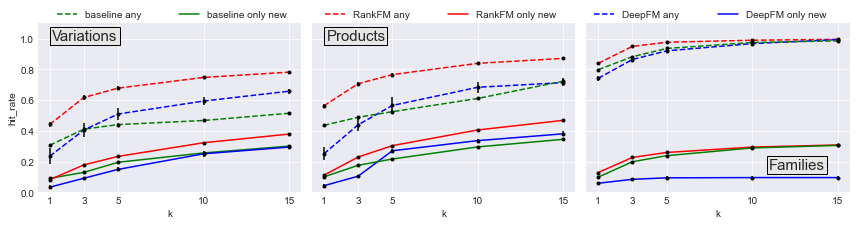
\includegraphics[width=\linewidth]{hit_rate.png}
	\caption{\textbf{Hit-rate and standard error} for baseline, RankFM and DeepFM for different number (k) of \textbf{any} (dashed line) and \textbf{only new} (full line) recommended \textbf{variations, products and families} separately.}
	\label{5}
\end{figure*}

\vspace*{-10pt}

\noindent In Table~\ref{tab:hyper-corr} we can see that embedding dimension (k) for all model is approx. 50 for all models, this indicates that there is a large amount of redundancy between features such as customer id and product id, both of which have over 1000 distinct values.
The low embedding dimension also leads us to assume that clusters should be present and clustering should be possible, since embedding dimension of above 100 are common for many machine learning task such as NLP.
Additionally, it appears that all 3 models require a fair bit of regularization. 
This can be achieved by using a large L2 regularization constant (RankFM), a large dropout rate (DeepFM) or a small learning rate (2nd order FM and DeepFM).
Finally, L1 regularization term was zero for both 2nd order FM and DeepFM is zero.
Considering L1 regularization performs feature selection, this would indicate that our dataset has no redundant features.

%\subsection*{Comparison of libraries vs implemented models}
%In this section we compare RankFM with our  1st and 2nd order FM implementations to analyze whether the flexiblity offered by our models improves our prediction accuracy or not.
%From Figure~\ref{hit_rate-custom} we conclude that the added flexibility achieved by implementing our models is overshadowed by many implemented optimisation present in popular libraries.

%\begin{figure}[H]\centering
%	\includegraphics[width=\linewidth]{final_hit_rate.png}
%	\caption{\textbf{Hit-rate and standard error} for RankFM and custom 1st and 2nd order FM's for different number (k) of %\textbf{any} and \textbf{only not previously bought} recommended  \textbf{variations}.}
%	\label{hit_rate-custom}
%\end{figure}

\subsection*{Hit-rate}

In Figure \ref{5} we show how our models perform compared to the baseline for different number of recommended items. We show hit-rates for both predicting any items and new, not yet purchased items by the individual customer. We split the plots into predicting \textbf{variations}, \textbf{products} and \textbf{families}. The more items we recommend the better the hit-rate. Since there are more different variations and products than families and customers are more likely to buy from the same family, hit-rate is the highest when predicting families and the lowest when predicting new families. We observe that RankFM outperforms the baseline and DeepFM in all possible combinations. DeepFM outperforms baseline only when recommending more than 5 any items and struggles to perform when recommending only new items.

% All three models managed to perform well and depending
%------------------------------------------------

\subsection*{F1-score}

\begin{figure}[H]\centering
	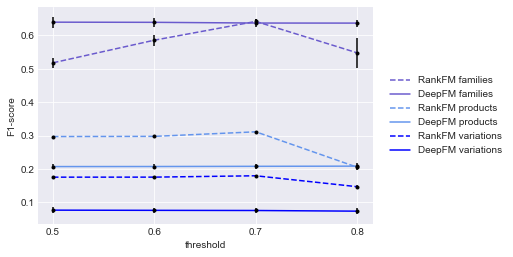
\includegraphics[width=\linewidth]{f1.png}
	\caption{\textbf{F1-score and standard error} for \textbf{RankFM} (dashed lines) and \textbf{DeepFM} (full lines) for recommending variations, products and families for different thresholds. Maximum number of recommended items was capped at 10.}
	\label{f1}
\end{figure}

In Figure \ref{f1} we show how F1-score changes based on chosen threshold for RankFM and DeepFM models. The F1-score improves only for RankFM family, while appearing constant or decreasing for all other models. More in-dept analysis showed F1-score was slightly increasing elsewhere as well, but is not noticeable on the plot. After we reach a threshold where we filter out correctly predicted items we observe a decrease in F1-score.

\section*{Conclusion}
%All algorithms improve upon the baseline, with RankFM improving the most due to most likely some optimal negative sampling method.
Our results have shown that due to customer tendencies to buy the same products, all three models predicting families give good results including the baseline model. Nevertheless, all algorithms improve upon the baseline, with RankFM achieving best performance regardless of number of recommended items. We observe a hit rate increase with number of predicted items for all models. The most significant improvement of the baseline model was accomplished by RankFM for variation and product prediction with hit@5 and hit@10.
% The RankFM gave us the best results with a hit@5 rate of 0.66 indicating that the customer will on average be interested in buying 3-out-5 product in our top@5 predictions, while DeepFM had a hit@5 rate of 0.51.

Thresholding was analysed using F1-score to take into account both precision and recall.
%From Figure~\ref{f1} it would appear all models can be improved using thresholding, however one needs to perform a line across different thresholds to find the optimum as its position varies depending on the algorithm used.
Thresholding improved F1-score only for RankFM family while increases were not substantial for other models.
This means that thresholding cannot be used to improve F1-score for product and variation.

Hyperparameter search was shown to improve model performance by a couple of percent for all models, indicating that GridSearch or some other more sophisticated method such as Bayesian Optimisation should be used since even a small increase in hit rate can result in larger amounts of sold products and therefore higher revenue over time.

We conclude that RankFM is the best performing model, while both RankFM and DeepFM perform better than the baseline indicating that the difference in performance is truly due to some optimisations in the RankFM library, rather than errors in our code.


%------------------------------------------------

%\section*{Acknowledgments}

%----------------------------------------------------------------------------------------
%	REFERENCE LIST
%----------------------------------------------------------------------------------------
\vspace*{-15pt}
\bibliographystyle{unsrt}
\bibliography{report}


\end{document}
